\documentclass[11pt]{beamer}

% Load template files
% Packages
\usepackage[T1]{fontenc}
\usepackage[utf8]{inputenc}
\usepackage{amsmath,amssymb}
\usepackage[right]{eurosym}
\usepackage{epstopdf}
\usepackage{graphicx}
\usepackage{rotating}
\usepackage{subfigure}
\usepackage{color}
\usepackage{xcolor}
\usepackage{colortbl}
\usepackage{moreverb}
\usepackage{eurosym}
\usepackage{booktabs}
\usepackage{textcomp}
\usepackage{lmodern}
\usepackage[dvipsnames]{pstricks}
\usepackage[absolute,overlay]{textpos}
\usepackage{listings} %for program code
\usepackage{tikz}
\usepackage{verbatim}
\usepackage{url}
\usepackage{hyperref}

% BIBLIOGRAPHY
%\usepackage[backend=biber,style=mla]{biblatex}
% Bib style
\usepackage[
	backend=biber,
	style=authoryear,
	sorting=nyt,
	natbib=true,
	url=false,
	eprint=false,
	isbn=false,
	maxcitenames=2,
	uniquename=init,  % disambiguate authors with same initials
	giveninits=true,  % only 1st letter of first name
	date=year,
]{biblatex}
\addbibresource{library.bib} % Name of your .bib file
%\addbibresource{/home/admin-tarassow/Nextcloud/thb_bwsyncandshare/LiteraturVerwaltung/library.bib} % Name of your .bib file
%\usepackage{natbib}


% Beamer settings
\usecolortheme{beaver}
\usetheme{CambridgeUS} % https://deic.uab.cat/~iblanes/beamer_gallery/index_by_theme.html

\setbeamercovered{transparent}
\setbeamertemplate{footline}[page number]
\setbeamertemplate{caption}[numbered] % Number the captions such as figures
\setbeamertemplate{navigation symbols}{}  % hide navigation symbols

% Settings for listings
\lstset{showstringspaces=false}

% THB specific Colors
\definecolor{THBRed}{RGB}{206,22,40}
\definecolor{THBBlue}{RGB}{22,132,206}
\definecolor{THBGreen}{RGB}{22,206,95}

% Python listing style
% For details: https://nasa.github.io/nasa-latex-docs/html/examples/listing.html
\lstdefinestyle{python}{
	language=python,
	basicstyle=\ttfamily\small,
	breakatwhitespace=false,  % sets if automatic breaks should only happen at whitespace
	breaklines=true,    % sets automatic line breaking
	captionpos=t,
	keepspaces=true,
	showlines=false,          % hide empty first/last listing lines
	numbers=left,
	numberblanklines=false,
	xleftmargin=1.5mm,   % left margin for code block
	xrightmargin=1.5mm,  % right margin for code block
	numbersep=5pt,
	showspaces=false,   % show spaces everywhere adding particular underscores; it overrides 'showstringspaces'
	showstringspaces=false,  % underline spaces within strings only
	showtabs=false,
	tabsize=2,
	frame=single,                % adds a frame around the code
	keywordstyle=\color{THBRed},
	% pandas-specific emphasis (listings is lexical, not semantic)
	emph={pd,DataFrame,Series,Index,read_csv,read_excel,head,tail,info,dtypes,isnull,fillna,astype,rename,columns,groupby,value_counts,nunique,unique,between,mean,sum,sort_values,copy,dropna,plt,figure,subplots,plot,scatter,hist,bar,barplot,lineplot,relplot,pairplot,boxplot,violinplot,heatmap,sns,sklearn,train_test_split,LinearRegression,LogisticRegression,DecisionTreeClassifier,RandomForestClassifier,KMeans,StandardScaler,MinMaxScaler,fit,transform,fit_transform,predict,score,classification_report,confusion_matrix,accuracy_score,mean_squared_error,r2_score},
	emphstyle=\color{THBBlue}\bfseries,
	commentstyle=\color{THBGreen},
	extendedchars=false
}

% Hansl/Gretl listing style
\lstdefinestyle{hansl}{
	language=hansl,
	basicstyle=\ttfamily\small,
	breakatwhitespace=false,  % sets if automatic breaks should only happen at whitespace
	breaklines=true,    % sets automatic line breaking
	captionpos=t,
	keepspaces=true,
	numbers=left,
	xleftmargin=1.5mm,   % left margin for code block
	xrightmargin=1.5mm,  % right margin for code block
	showlines=false,          % hide empty first/last listing lines
	numberblanklines=false,
	numbersep=5pt,
	showspaces=false,   % show spaces everywhere adding particular underscores; it overrides 'showstringspaces'
	showstringspaces=false,  % underline spaces within strings only
	showtabs=false,
	tabsize=2,
	frame=single,                % adds a frame around the code
	keywordstyle=\color{THBRed},
	commentstyle=\color{THBGreen},
	extendedchars=false
}

% Default to Python style
\lstset{style=hansl}
% Important: keep \end{lstlisting} at the beginning of the line.
% Leading spaces before \end{lstlisting} are treated as an extra (empty) code line.

% Custom commands and environments
\hypersetup{
	colorlinks=true,
	urlcolor=blue,
	citecolor=mygreen,
	linkcolor=blue,
}

% Information to be included in the title page:
\logo{
\includegraphics[height=0.8cm]{THB_FB-W_Logo.jpg}\vspace{220pt}}

\author[Tarassow]{Artur Tarassow}
% - Use the \inst command only if there are several affiliations.
% - Keep it simple, no one is interested in your street address.
\institute{
	\inst{} Applied University of Brandenburg
	\newline
	\texttt{\small{artur.tarassow@th-brandenburg.de}}
}


%%%%%%%%%%%%%%%%%%%%%%%%%%%%%%%%%%%%%%%%%%%%%%%%%%%%
%%% VON DANIEL
%%%%%%%%%%%%%%%%%%%%%%%%%%%%%%%%%%%%%%%%%%%%%%%%%%%%
%              cmsst_header.tex
%
% Fonts:
%
%\usepackage{eulervm}
%\usepackage[scaled]{helvet}
%\def\normalsize{\fontsize{12bp}{14bp}\selectfont}

\newtheorem{defi}{Definition}%[chapter]
\newcommand{\E}{\mathop{\mathbb E}} %% Expectation operator

% colors
\definecolor{mygreen}{rgb}{0.0,0.5,0.0}
\definecolor{myred}{rgb}{0.9,0,0}
\newcommand{\remph}[1]{{\color{myred}#1}}
\definecolor{THBRed}{RGB}{206,22,40}
\definecolor{THBBlue}{RGB}{22,132,206}
\definecolor{THBGreen}{RGB}{22,206,95}


% Title slide information
\title{Introduction to Time Series Forecasting}
\subtitle{Practical Methods and Applications}
\date{Ancona Erasmus Lecture}

%***********************************************************************************************

\begin{document}

\begin{frame}
	\titlepage
\end{frame}

\begin{frame}[fragile]{Outline}
	\tableofcontents
\end{frame}

\begin{frame}[fragile]{References}
	\begin{itemize}
		\item \citet{hyndman2021ForecastingPrinciplesPractice}, URL: \url{https://otexts.com/fpp3/}
		\begin{itemize}
			\item Gretl Replication Files: \url{https://github.com/gretl-project/forecasting_principles}
		\end{itemize}
		\item \citet{castelForecastingEssentialIntroduction2019}
		\item \citet{diebold2024ForecastingEconomicsBusiness}
		\item \citet{elliott2016EconomicForecasting}
		\item \citet{enders2015AppliedEconometricTime}
	\end{itemize}
\end{frame}

% ==================== SECTION 1: INTRODUCTION ====================

\section{Introduction to Forecasting}

\begin{frame}
	\begin{center}
		\Large
		Introduction to Forecasting
		\vspace{1cm}

		\textit{``A forecast is any statement about the future.''}
		\vspace{0.25cm}

		\scriptsize{\citet{castelForecastingEssentialIntroduction2019}}
	\end{center}
\end{frame}

\begin{frame}[fragile]{What is Forecasting and Why Does It Matter?}
	\begin{block}{Forecast}
		Seeks to predict the future as accurately as possible, taking into account all available information, including historical data and knowledge of future events that may influence forecasts. \scriptsize{\citet{hyndman2021ForecastingPrinciplesPractice}}
	\end{block}

	\begin{itemize}
		\setlength{\itemsep}{0.25cm}
		\item Forecasting is integral to decision-making in business and economics.
		\item \textbf{Business:} supports operations, staffing, finance, and strategy.
		\item \textbf{Economics:} informs GDP, inflation, unemployment, and policy planning.
		\item Forecast horizons depend on purpose:
		\begin{itemize}
			\item \textbf{Short-term}: operational control
			\item \textbf{Medium-term}: budgeting and capacity planning
			\item \textbf{Long-term}: investment and strategic/policy direction
		\end{itemize}
	\end{itemize}
\end{frame}

% \begin{frame}[fragile]{Forecasting in Practice}
% 	\begin{itemize}
% 		\setlength{\itemsep}{0.25cm}
% 		\item Building another power plant $\rightarrow$ Requires forecasts of future demand.
% 		\item Personnel planning in a call center $\rightarrow$ Requires forecasts of call volumes.
% 		\item Inventory management $\rightarrow$ Requires forecasts of stock levels.
% 		\item Forecast horizon can vary widely: from
% 		\begin{itemize}
% 			\item several years in advance (capital investments),
% 			\item only minutes before (for telecommunications routing).
% 		\end{itemize}
% 		\item \textbf{Forecasts are an important aid for effective and efficient planning}.
% 	\end{itemize}
% 	%\medskip
% 	%More examples: \url{https://otexts.com/fpp3/case-studies.html}
% \end{frame}

\begin{frame}[fragile]{Predictability: What Determines It?}
	\begin{enumerate}
		% set space between items to 0.5cm
		\setlength{\itemsep}{0.5cm}
		\item How well we understand the factors that contribute;
		\item How much data is available;
		\item How similar the future is to the past (structural stability);
		\item Whether forecasts can influence what we are trying to predict (self-fulfilling prophecies).
	\end{enumerate}
\end{frame}

\begin{frame}[fragile]{Short-term Electricity Demand Forecasts...}
	...can be forecast accurately because all \textbf{four predictability conditions} are usually met:
	\begin{itemize}
		\setlength{\itemsep}{0.2cm}
		\item[$\checkmark$] Good understanding of contributing factors: Temperature, with minor effects from calendar deviations like holidays and economic conditions.
		\item[$\checkmark$] Long history: Multiple years of electricity demand data are  available, along with decades of weather data.
		\item[$\checkmark$] Structural stability: For short-term forecasts, we can assume stable demand behavior.
		\item[$\checkmark$] No feedback effects: Demand forecasts have little or no influence on consumer behavior.
	\end{itemize}
\end{frame}

\begin{frame}[fragile]{Exchange Rate Forecasts Are More Difficult}
	\begin{itemize}
		\setlength{\itemsep}{0.2cm}
		\item[$\checkmark$] Plenty of available data.
		\item[$\times$] Deep understanding of factors influencing exchange rates.
		\item[$\times$] The future mimics the past only to a high extent.
		\item[$\times$] Public forecasts have no effect on the exchange rate.
	\end{itemize}
	\medskip

	\textbf{Result:} Exchange rate forecasts are often inaccurate. This is consistent with the \textbf{random walk hypothesis} in finance, which states that exchange rates follow a random walk and are therefore unpredictable.
\end{frame}



\begin{frame}[fragile]{The Forecasting Workflow}
	\begin{columns}
		\column{0.4\textwidth}
		\small
		\begin{enumerate}
			\item \textbf{Collect \& Clean}: Collect and preprocess data
			\item \textbf{Exploratory Analysis}: Understand data patterns
			\item \textbf{Model Selection}: Choose appropriate method
			\item \textbf{Estimation}: Fit model to training data
			\item \textbf{Evaluation}: Assess accuracy on test data
			\item \textbf{Forecasting}: Generate predictions
		\end{enumerate}

		\column{0.6\textwidth}
		\begin{figure}
			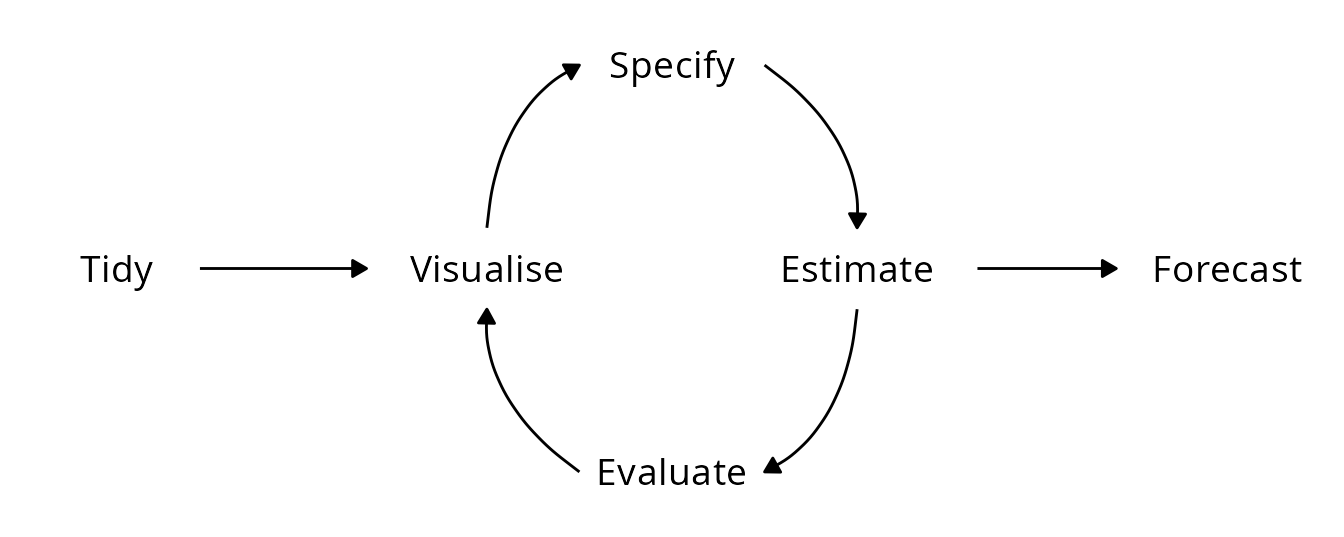
\includegraphics[width=0.9\textwidth]{../figures/fpp_tidy_forecasting_workflow.png}
		\end{figure}
	\end{columns}
\end{frame}

\begin{frame}[fragile]{Key Concepts}
	\begin{itemize}
		\item \textbf{Point Forecast}: Single predicted value
		      \begin{itemize}
			      \item Example: ``GDP growth next quarter = 2.5\%''
		      \end{itemize}

		\item \textbf{Prediction Interval}: Range of plausible values
		      \begin{itemize}
			      \item Example: ``GDP growth 95\% CI: [1.8\%, 3.2\%]''
		      \end{itemize}
		\item \textbf{Probabilistic Forecast}: Full distribution of future values
		      \begin{itemize}
			      \item Example: ``GDP growth has 30\% chance of being above 2\%''
		      \end{itemize}

		\item \textbf{Training Data}: Used to fit the model

		\item \textbf{Test Data}: Held out to evaluate forecast accuracy

		\item \textbf{In-sample vs. Out-of-sample}:
		      \begin{itemize}
			      \item In-sample fit does NOT guarantee good forecasts (overfitting)
		      \end{itemize}

		\item \textbf{Naive/simple vs. Sophisticated Methods}:
		      \begin{itemize}
			      \item Always compare to simple benchmarks (e.g., mean, last value)
			      \item Sophisticated methods must outperform naive ones to be useful
			      \item Simple methods are often hard to beat, especially for short-term forecasts
		      \end{itemize}
	\end{itemize}
\end{frame}

% ==================== SECTION 2: NAIVE METHODS ====================

\section{Naive Forecasting Methods}

\begin{frame}
	\begin{center}
		\Large
		Naive Forecasting Methods
	\end{center}
\end{frame}

\begin{frame}{Why Start with Naive Methods?}
	\begin{itemize}
		\setlength{\itemsep}{0.25cm}
		\item \textbf{Benchmark}: Any sophisticated method should beat naive forecasts or simple forecasting methods
		\item \textbf{Interpretability}: Easy to understand and explain
		\item \textbf{Practical}: Often surprisingly effective --- at least as useful benchmarks
		\item \textbf{Big-Data}: Applying naive methods to \textit{zillions} of time series (e.g., retail sales by product) can be done in reasonable time and often even by SQL queries.
	\end{itemize}
	\vspace{1cm}
	Read also Rob J Hyndman's blog post on the relevance of benchmarks: \url{https://robjhyndman.com/hyndsight/benchmarks}
\end{frame}

\begin{frame}{Mean Method}
	\textbf{Forecast all future values as the historical average:}
	\begin{equation}
		\hat{y}_{T+h|T} = \bar{y} = \frac{1}{T}\sum_{t=1}^{T} y_t
	\end{equation}
	for historical data $y_1, y_2, \ldots, y_T$.

	\vspace{0.5cm}
	\textbf{When to use:} Stationary data without trend, seasonality and minor persistence.
	\medskip

	\textbf{Robust version}: Median method (forecast = median of historical data) is more robust to outliers.
\end{frame}

\begin{frame}{Naïve Method (Random Walk)}
	\textbf{Forecast: the last observed value}
	\begin{equation}
		\hat{y}_{T+h|T} = y_T
	\end{equation}

	%\vspace{0.5cm}
	%\textbf{Gretl implementation:}
	%\begin{verbatim}
		%series yhat = y[T]  # constant at last value
	%\end{verbatim}

	\vspace{0.5cm}
	\textbf{When to use:} Random walk data (most economic/financial series)
	\begin{itemize}
		\item Stock prices, exchange rates, unit root processes
		\item Adapts to level shifts and trends automatically
	\end{itemize}
\end{frame}

\begin{frame}{Random Walk plus Drift Method}
	\textbf{Forecast: last value plus average historical change}
	\begin{equation}
		\hat{y}_{T+h|T} = y_T + h \underbrace{\left(\frac{y_T - y_1}{T-1}\right)}_{\text{average change}}
	\end{equation}

	\vspace{0.5cm}
	\textbf{Interpretation:} Extrapolate linear trend from first to last observation

	\vspace{0.5cm}
	%\textbf{Gretl implementation:}
	%\begin{verbatim}
	%scalar trend = (y[T] - y[1]) / (T - 1)
	%series yhat = y[T] + trend * seq(1, h)
	%	\end{verbatim}

	\vspace{0.5cm}
	\textbf{When to use:} Data with steady trend (GDP, population, cumulative sales)
\end{frame}

\begin{frame}{Seasonal Naïve Method}
	\textbf{Forecast: last observed value from same season}
	\begin{equation}
		\hat{y}_{T+h|T} = y_{T+h-m(k+1)}
	\end{equation}
	where $m$ = seasonal period (e.g., 4 for quarterly, 12 for monthly), and $k$ is the integer part of $(h-1)/m$ (i.e., the number of complete years in the forecast period prior to time $T+h$).

	\vspace{0.5cm}
	\textbf{Example:} For quarterly data, forecast Q2 2024 = Q2 2023 value

	\vspace{0.5cm}
	\textbf{When to use:} Highly seasonal data without trend (retail sales, tourism, energy)
\end{frame}


\begin{frame}{Seasonal Mean Method}
    \textbf{Idea:} Forecast using the historical mean of the corresponding season.

    \begin{equation}
        \hat{y}_{T+h|T} = \bar{y}_{s(T+h)}
        \quad\text{with}\quad
        \bar{y}_{j}=\frac{1}{N_j}\sum_{t\in \mathcal{S}_j} y_t
    \end{equation}

    \begin{itemize}
        \item \textbf{Weekday frequency:} one mean for each weekday
        \item \textbf{Monthly frequency:} one mean for each month (12 means)
        \item \textbf{Quarterly frequency:} one mean for each quarter (4 means)
    \end{itemize}

    \textbf{When useful:} Stable seasonal pattern, weak trend.
\end{frame}


\begin{frame}[fragile]{Comparing the Methods}
	\begin{figure}
		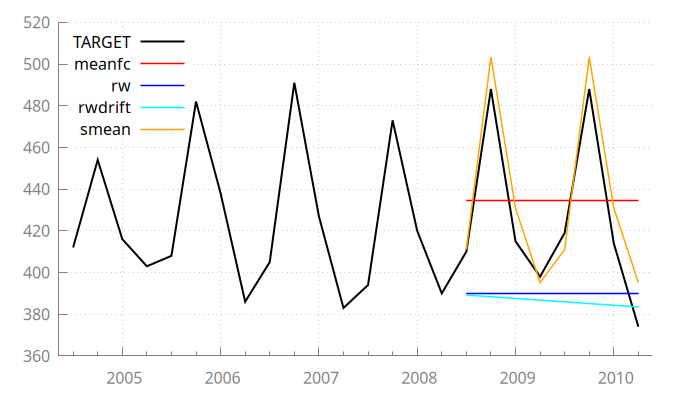
\includegraphics[width=0.75\textwidth]{../figures/comparison_naive_methods.png}
		\caption{Australian quarterly beer production: Mean, Random Walk, Random Walk + Drift and Seasonal Mean forecasts}
	\end{figure}
\end{frame}


\begin{frame}[fragile]{When Do Naive Methods Fail?}
	\begin{itemize}
		\item Data with \textbf{autocorrelation}: Past values contain predictive info
		\item \textbf{Complex patterns}: Trends, level shifts, cycles
		\item \textbf{Structural dependencies}: Future depends systematically on past
	\end{itemize}

	\vspace{0.5cm}
	\textbf{More advanced time-series models:}
	\begin{itemize}
		\item (S)ARIMA(X)
		\item Exponential Smoothing
		\item Regression with ARMA errors (ARIMAX)
		\item ARDL and VAR
		\item Structural Time Series Models (e.g., unobserved components)
		\item Etc.
	\end{itemize}

\end{frame}

\begin{frame}{Naive/simple Methods Using Gretl}
	Gretl provides all relevant functions for computing naive methods.
	\vspace{0.3cm}

	Make use of the `arima` and `ols` commands.\footnote{See relevant chapters in the User's Guide. URL: \url{https://gretl.sourceforge.net/gretl-help/gretl-guide.pdf}}
	\vspace{0.3cm}

	The ``naiveFC'' package provides a convenient interface for generating forecasts from naive methods, including point forecasts and prediction intervals:
	\begin{itemize}
		%\item Support for 10 different naive methods
		%\item Moving-window for rolling and recursive multi-step forecasts
		\item Doc: \url{https://gretl.sourceforge.net/current_fnfiles/unzipped/naiveFC.pdf}
		\item Github: \url{https://github.com/atecon/naiveFC/tree/master/}
		\item Package needs some update, but works
	\end{itemize}
\end{frame}



\section{Time Series Regression Models}

\begin{frame}
	\begin{center}
		\Large
		Time Series Regression Models\\
		---\\
		Some useful predictors
	\end{center}
\end{frame}

\begin{frame}[fragile]{Trend Regression}
	\textbf{Definition:} Model linear trends in time series data

	\vspace{0.2cm}
	\textbf{Model:}
	\begin{equation}
		y_t = \beta_0 + \beta_1 \cdot t + \varepsilon_t \quad t=1, 2, \ldots, T
	\end{equation}

	\begin{columns}[T]
        \column{0.35\textwidth}
        \begin{itemize}
			\item $\beta_0$: Starting level
			\item $\beta_1$: Average change per time period
            \item \textbf{When to use:} Trend stationary series with deterministic trend
        \end{itemize}

        \column{0.65\textwidth}
        \begin{figure}
            \centering
            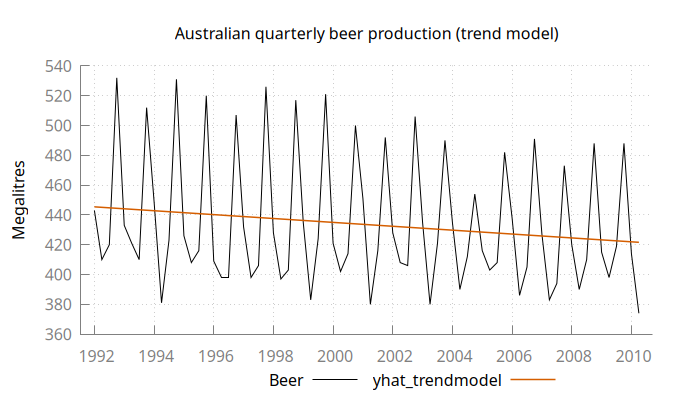
\includegraphics[width=0.85\textwidth]{../figures/trend_model_actual_fitted.png}
            \caption{In-sample fit of trend regression model to Australian beer production data}
        \end{figure}
    \end{columns}
\end{frame}


\begin{frame}[fragile]{Dummy Variables for Categorical Effects}
	Encode categorical information into regression models.

	\vspace{0.3cm}
	\textbf{Common uses:}
	\begin{itemize}
		\item \textbf{Holidays/Special events}: Public holidays\footnote{See the gretl package ``holidays'' for built-in holiday calendars: \url{https://gretl.sourceforge.net/current_fnfiles/holidays.gfn}.}, Sport events
		\item \textbf{Intervention effects}: Marketing campaigns, policy changes
		\item \textbf{Outliers}: Handle special one-time events
	\end{itemize}

	%\vspace{0.3cm}
	%\textbf{Key rule -- The ``Dummy Variable Trap'':}
	%\begin{itemize}
	%	\item For $k$ categories, use \textbf{exactly $(k-1)$ dummy variables}
	%	\item The omitted category is captured by the intercept
	%	\item Including all $k$ dummies causes multicollinearity
	%\end{itemize}

	\vspace{0.3cm}
	\textbf{Interpretation:} Each coefficient represents the effect \textbf{relative to the reference (omitted) category}
\end{frame}

\begin{frame}{Seasonal Dummy Variables}
	%\textbf{Seasonal patterns as categorical variables:}
	Example: \textbf{Quarterly} with 4 categories $\Rightarrow$ use 3 dummy variables

	\vspace{0.3cm}
	\begin{center}
		\small
        \begin{tabular}{ccccc}
            \toprule
            Quarter & $d_{1,t}$ & $d_{2,t}$ & $d_{3,t}$ \\
            \midrule
            Q1      & 1         & 0         & 0         \\
            Q2      & 0         & 1         & 0         \\
            Q3      & 0         & 0         & 1         \\
            Q4      & 0         & 0         & 0         \\
            \bottomrule
        \end{tabular}
	\end{center}

	\vspace{0.15cm}
	\textbf{Extensions} -- handle different seasonalities\footnote{Fourier series (sine and cosine terms) provide an alternative for modelling seasonality, especially useful for long seasonal periods. See \url{https://otexts.com/fpp3/dhr.html} for details.}
	\begin{itemize}
		\item \textbf{Weekly data:} 6 dummies (for Mon, ..., Sat; Sun is reference)
		\item \textbf{Monthly data:} 11 dummies (for Jan--Nov; Dec is reference)
	\end{itemize}
\end{frame}

\begin{frame}{Seasonal Model plus linear Trend}
	\textbf{Model example:} (quarterly frequency)  $$y_t = \beta_0 + \beta_1 t + \beta_2 d_{2,t} + \beta_3 d_{3,t} + \beta_4 d_{4,t} + \varepsilon_t$$

	% two figures side-by-side (subplot)
	\begin{figure}
		\begin{minipage}{0.475\textwidth}
			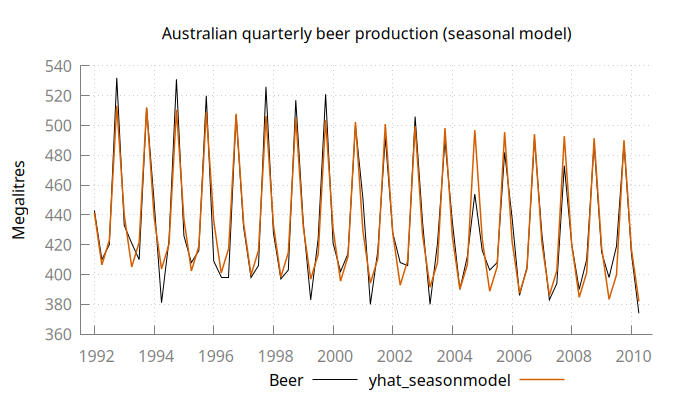
\includegraphics[width=\textwidth]{../figures/seasonal_model_actual_fitted.png}
			\caption{In-sample fit of seasonal regression model}
		\end{minipage} %\hfill
		\begin{minipage}{0.475\textwidth}
			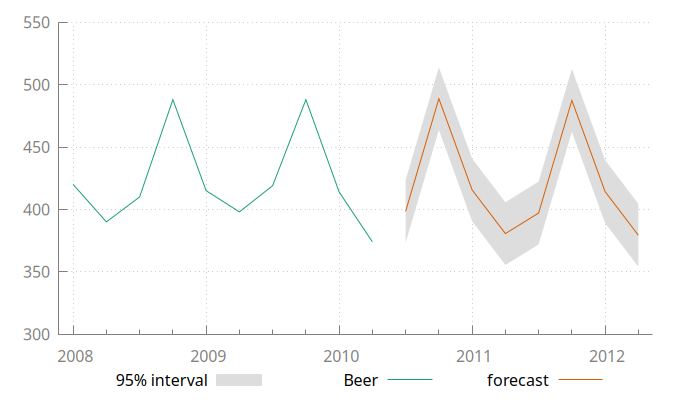
\includegraphics[width=\textwidth]{../figures/seasonal_model_forecast_with_intervals.png}
			\caption{Out-of-sample forecast with prediction intervals}
		\end{minipage}
	\end{figure}
\end{frame}


\begin{frame}[fragile]{Distributed Lags: Modeling Lagged Effects}
	\textbf{Motivation:} Some predictors have effects lasting multiple time periods

	\vspace{0.2cm}
	\textbf{Example:} Advertising campaign
	\begin{itemize}
		\item Sales impact occurs not only in the campaign month, but also in subsequent months $\rightarrow$ Need to capture cumulative/delayed effects
	\end{itemize}

	\vspace{0.2cm}
	\textbf{Distributed lag model:}
	$$y_t = \beta_0 + \beta_1 X_{t-1} + \beta_2 X_{t-2} + \cdots + \beta_m X_{t-m} + \varepsilon_t$$

	where $X_{t-j}$ is the predictor value $j$ periods in the past.

	%\vspace{0.2cm}
	%\textbf{Interpretation:} $\beta_j$ measures the effect of the predictor $j$ periods ago

	\vspace{0.2cm}
	\textbf{Forecasting Challenge:}
	\begin{itemize}
		\item To forecast $y_{T+h}$, we need values $X_{T+h-1}, X_{T+h-2}, \ldots, X_{T+h-m}$
		\item Many of these future $X$ values are \textbf{unknown}
		\item Must either: (1) use assumptions about future $X$, or (2) forecast $X$ as well
		\item Makes out-of-sample forecasting more difficult and uncertain
	\end{itemize}
\end{frame}


\begin{frame}{Distributed Lags: Example with Beer and Cement}
	\textbf{Model example:} $$Beer_t = \beta_0 + \beta_1 time + \beta_2 \text{Cement}_{t-6} + \beta_3 \text{Cement}_{t-7} + \beta_4 \text{Cement}_{t-8} + \varepsilon_t$$

	(You may also add a seasonal component if needed, but we focus on the distributed lag aspect here)

	% two figures side-by-side (subplot)
	\begin{figure}
		\begin{minipage}{0.475\textwidth}
			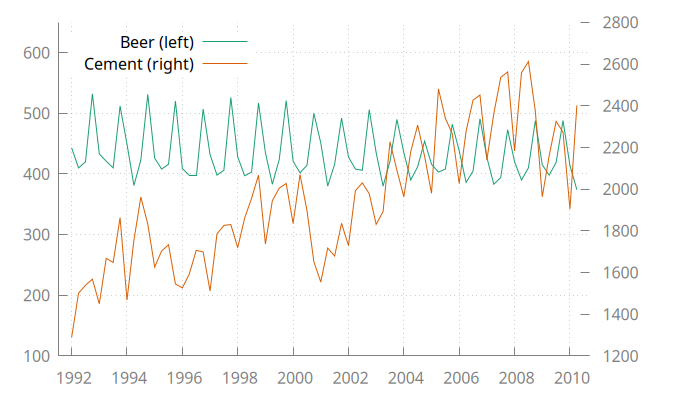
\includegraphics[width=\textwidth]{../figures/tsplot_beer_cement.png}
			\caption{Historical data for beer production and cement production}
		\end{minipage} %\hfill
		\begin{minipage}{0.475\textwidth}
			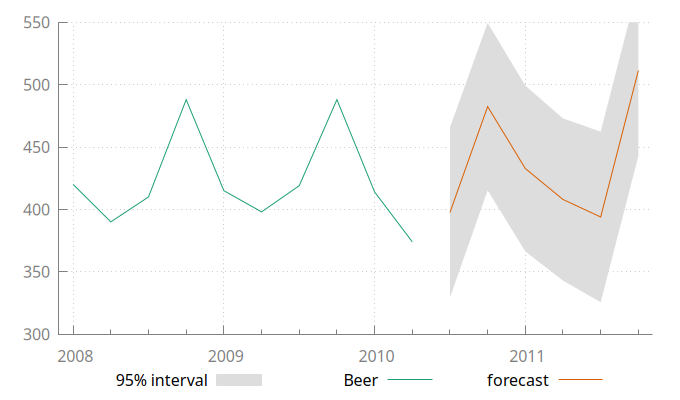
\includegraphics[width=\textwidth]{../figures/distributed_model_forecast_with_intervals.png}
			\caption{Out-of-sample forecast with prediction intervals}
		\end{minipage}
	\end{figure}
\end{frame}


% ==================== SECTION 3: PREDICTION INTERVALS ====================

\section{Forecast Intervals and Uncertainty}

\begin{frame}
	\begin{center}
		\Large
		Forecast Intervals and Uncertainty
	\end{center}
\end{frame}

\begin{frame}[fragile]{Why Prediction Intervals Matter}
	\begin{itemize}
		\item Point forecasts alone are incomplete
		\item Decision-makers need to know the \textbf{range of uncertainty}
		\item Narrow intervals $\Rightarrow$ more confident forecast
		\item Wide intervals $\Rightarrow$ high uncertainty
	\end{itemize}

	\vspace{0.5cm}
	\textbf{Example:}
	\begin{itemize}
		\item Bad: ``Sales will be \$100M''
		\item Better: ``Sales will be \$100M [95\% CI: \$80M--\$120M]''
	\end{itemize}

	\begin{figure}
		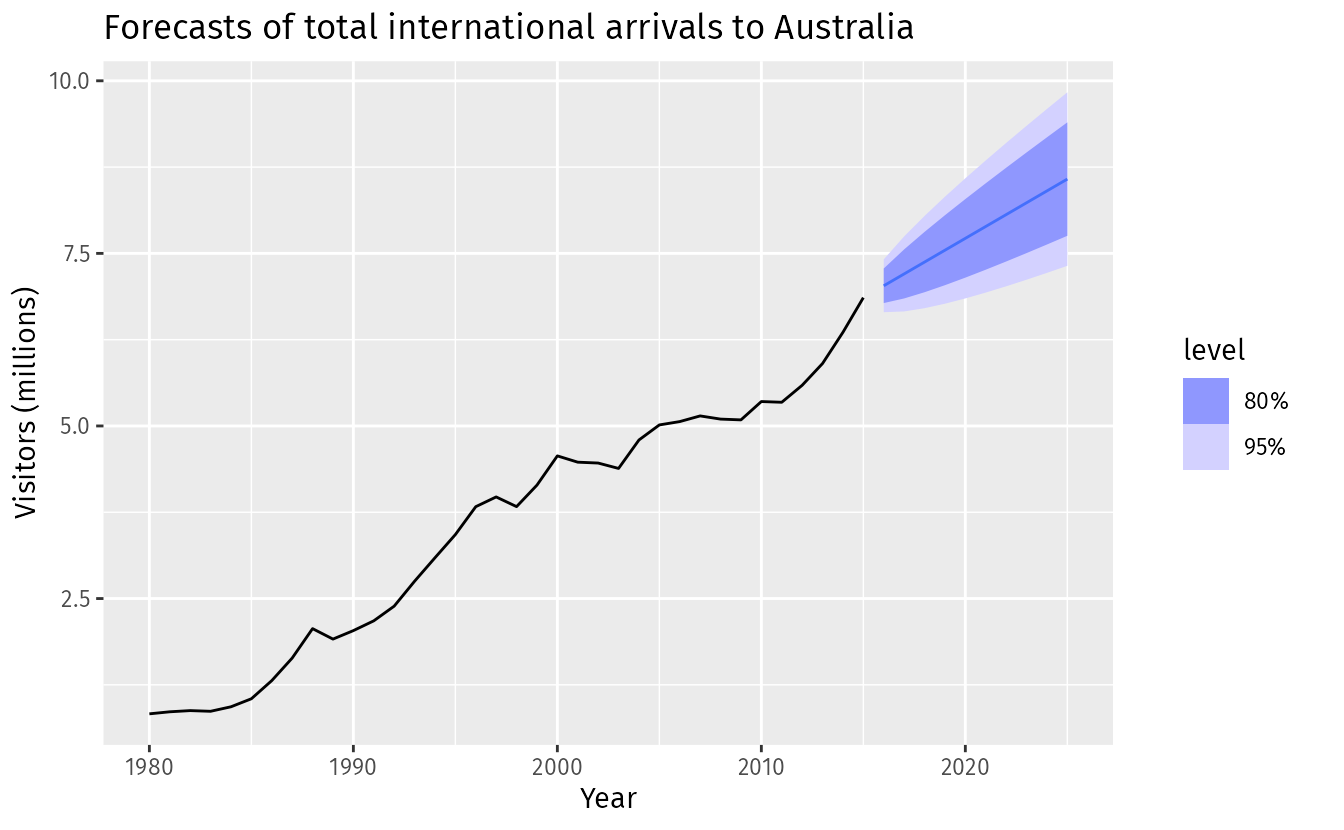
\includegraphics[width=0.5\textwidth]{../figures/hyndman_forecast_interval_example.png}
		\caption{Forecast with 80\% and 95\% prediction intervals}
	\end{figure}
\end{frame}

\begin{frame}[fragile]{Interpretation of Prediction Intervals}
	\textbf{80\% prediction interval:} If we repeat this forecast many times, the interval will cover actual values in about 80\% of the time.

	\vspace{0.5cm}
	\textbf{95\% prediction interval:} Higher coverage (wider band) for more confidence. Less useful for decision-making if too wide.

	\vspace{0.5cm}
	\textbf{Methods to construct intervals:}
	\begin{itemize}
		\item \textbf{Asymptotic}: Based on normality of residuals
		\item \textbf{Bootstrap}: Resampling from residuals (or forecast errors) (more robust)
	\end{itemize}

	\vspace{0.5cm}
	\textbf{Note:} Software packages typically provide interval estimates for classical models (e.g., ARIMA forecasts)
\end{frame}

\begin{frame}[fragile]{Benchmark Methods: Forecast Standard Deviations}
	\textbf{Mathematical foundation:} Derive $h$-step forecast uncertainty under uncorrelated residuals

	\vspace{0.3cm}
	Let $\hat{\sigma}_h$ = standard deviation of $h$-step forecast distribution, and $\hat{\sigma}$ = residual standard deviation

	\vspace{0.5cm}
	\begin{table}
		\small
		\centering
		\begin{tabular}{ll}
			\toprule
			\textbf{Benchmark Method} & \textbf{$h$-step Forecast Std Dev} \\
			\midrule
			Mean & $\hat{\sigma}_h = \hat{\sigma}\sqrt{1 + 1/T}$ \\
			Naïve & $\hat{\sigma}_h = \hat{\sigma}\sqrt{h}$ \\
			Seasonal Naïve & $\hat{\sigma}_h = \hat{\sigma}\sqrt{k+1}$ \\
			Drift & $\hat{\sigma}_h = \hat{\sigma}\sqrt{h\left(1 + \frac{h}{T-1}\right)}$ \\
			\bottomrule
		\end{tabular}\\
		\footnotesize Source: \url{https://otexts.com/fpp3/prediction-intervals.html}
	\end{table}

	\vspace{0.3cm}
	Alternatively: use bootstrap methods (no need to rely on distributional assumptions).
	%\textbf{Notation:} $m$ = seasonal period, $k$ = integer part of $(h-1)/m$ (complete years in forecast period)

	%\vspace{0.3cm}
	%\textbf{Key observation:} When $h=1$ and $T$ is large, all methods give approximately the same $\hat{\sigma}$
%
	%\vspace{0.3cm}
	%\textbf{Implication:} Forecast uncertainty increases with horizon; methods differ in rate of growth
\end{frame}

% ==================== SECTION 4: FORECAST EVALUATION ====================

\section{Forecast Evaluation}

\begin{frame}
	\begin{center}
		\Large
		Forecast Evaluation

		---

		Of Point Forecasts
	\end{center}
\end{frame}

\begin{frame}{Motivation}
    \begin{itemize}
        \item Performance on known data is not a good indicator of prediction performance on unknown data!
        \item \textbf{Overfitting}: A model that adapts too strongly to the training data.
        \item A useful model should be able to \textit{generalize}.
        \item \textbf{Generalization}: The ability of a model to predict on unknown data.
        \item \textbf{Cross-validation}: A method for estimating the generalization performance of a model.
        \item Evaluating \textit{out-of-sample} prediction performance provides a measure of model quality.
    \end{itemize}
    % \medskip

    % Performance is measured by the test error, either to:
    % \begin{enumerate}
    % 	\item \textbf{Model selection}: Estimate the performance of different models to select the best one.
    % 	\item \textbf{Model evaluation}: After a final model has been chosen, estimate its prediction error (generalization error) on new data.
    % \end{enumerate}
\end{frame}

\begin{frame}{Training and Test Errors}
    We distinguish between:
    \begin{enumerate}
        \item \textbf{Training error}: Residuals aka \textit{in-sample error}
        \item \textbf{Test (Generalization) error}: Forecast error when predicting unseen test data (\textit{out-of-sample} prediction).
    \end{enumerate}
    \medskip

    \textbf{Goal}: Minimize some loss function based on test error.
    \medskip

    The training error can dramatically underestimate the test error.
    \medskip

    For model selection and evaluation, we evaluate the test error.
\end{frame}


\begin{frame}[fragile]{Train-Test Split}
	\textbf{Why separate data?}
	\begin{itemize}
		\item Training data: Fit the model, estimate parameters
		\item Test data: Evaluate forecast accuracy on new data
		%\item For genius forecasts: Do not evaluate on training data!
	\end{itemize}

	\vspace{0.25cm}
	\textbf{Typical split:} 80\% training, 20\% test
	\begin{itemize}
		\item Depends on: Data length, forecast horizon
		\item Rule: Test set $\geq$ longest forecast horizon
	\end{itemize}

	\begin{figure}
        \centering
        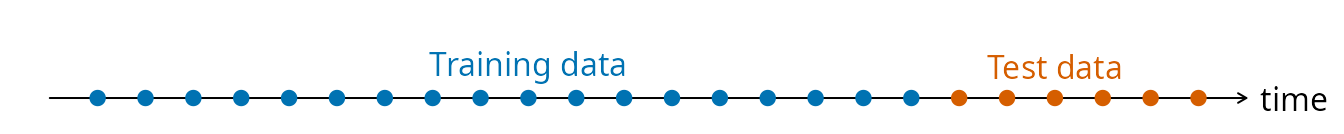
\includegraphics[width=0.9\textwidth]{../figures/hyndman_traintest.png}
        \caption{Train-test split for time series forecasting}
    \end{figure}

	\vspace{0.25cm}
	\textbf{Important:} Maintain temporal order (no random shuffling!)
\end{frame}

\begin{frame}[fragile]{Forecast Errors}
	\textbf{Definition:} Difference between observed and forecast value
	$$e_{T+h} = y_{T+h} - \hat{y}_{T+h|T}$$

	\vspace{0.5cm}
	\textbf{Key distinction:}
	\begin{itemize}
		\item \textbf{Residuals}: Errors on training data (one-step ahead)
		\item \textbf{Forecast errors}: Errors on test data (can be multi-step)
	\end{itemize}

	\vspace{0.5cm}
	\textbf{Why it matters:} Residuals underestimate true forecast uncertainty
\end{frame}

\begin{frame}{Example: Calculating Forecast Errors \& Metrics}
	\begin{figure}
		\centering
		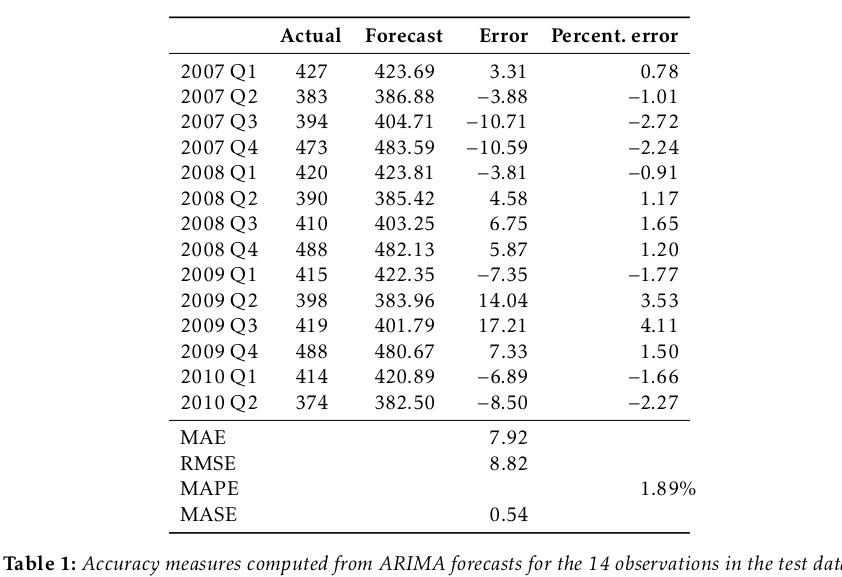
\includegraphics[width=0.8\textwidth]{../figures/Hyndman_Forecast_Eval_Example.png}
		\caption{14-$h$-step forecasts for \textit{one} training period. Source: \citet{hyndman2014MeasuringForecastAccuracy}}
	\end{figure}
\end{frame}


\begin{frame}[fragile]{Mean Error (ME) I: Forecast Bias}
    \textbf{Definition:} Average forecast error
    \begin{equation}
		\text{ME} = \text{mean}(e_t) \qquad \text{where} \quad  e_t = y_t - \hat{y}_{t}
	\end{equation}

    \vspace{0.4cm}
    \textbf{Interpretation (bias):}
    \begin{itemize}
        \item $\text{ME} > 0$: systematic \textbf{under-prediction} (forecasts too low)
        \item $\text{ME} < 0$: systematic \textbf{over-prediction} (forecasts too high)
        \item $\text{ME} \approx 0$: little average bias
    \end{itemize}

    \vspace{0.3cm}
    \textbf{Note:} ME can hide large errors due to cancellation, so combine with MAE/RMSE.
\end{frame}

\begin{frame}[fragile]{Error Metrics II: Scale-Dependent}
    \textbf{Mean Absolute Error (MAE):}
    \begin{equation}
        \text{MAE} = \text{mean}(|e_t|)
    \end{equation}
    \begin{itemize}
		\item Linear loss: Each unit of error contributes equally to total error
        \item Interpretation: Average absolute forecast error in original units
        %\item Good for single series or same units
    \end{itemize}

    \vspace{0.5cm}
    \textbf{Root Mean Squared Error (RMSE):}
    \begin{equation}
        \text{RMSE} = \sqrt{\text{mean}(e_t^2)}
    \end{equation}
    \begin{itemize}
        \item Quadratic loss: Penalizes large errors more heavily
        \item Also in original units
    \end{itemize}

    \vspace{0.5cm}
    \textbf{When to use:} Comparing methods on same series
\end{frame}

\begin{frame}[fragile]{Error Metrics III: Percentage-Based}
	\textbf{Mean Absolute Percentage Error (MAPE):}
	$$\text{MAPE} = \text{mean}(|p_t|) \quad \text{where} \quad p_t = \frac{100 \times e_t}{y_t}$$
	\begin{itemize}
		\item Unit-free: Compare across series with different scales
		\item Problem: Undefined if $y_t = 0$; biased if $y_t$ near zero
	\end{itemize}

	\vspace{0.5cm}
	\textbf{Further Material:}
	\begin{itemize}
		\item More metrics: \url{https://otexts.com/fpp3/accuracy.html}
		\item Metrics for probabilistic forecasts: \url{https://otexts.com/fpp3/distaccuracy.html}
	\end{itemize}
\end{frame}

% \begin{frame}[fragile]{Error Metrics III: Scaled Errors (Modern Approach)}
% 	\textbf{Mean Absolute Scaled Error (MASE):}
% 	$$\text{MASE} = \text{mean}\left(\left|\frac{e_j}{\frac{1}{T-1}\sum_{t=2}^T |y_t - y_{t-1}|}\right|\right)$$

% 	\vspace{0.3cm}
% 	\begin{itemize}
% 		\item Scales errors by training MAE of naive forecast
% 		\item MASE < 1: Better than naive method
% 		\item MASE > 1: Worse than naive method
% 		\item Unit-free and scale-independent
% 	\end{itemize}

% 	\vspace{0.5cm}
% 	\textbf{Advantage:} Can compare different series/units \citep{hyndman2014MeasuringForecastAccuracy}

% 	\vspace{0.3cm}
% 	\textbf{Recommendation:} Use MASE as primary metric for comparison
% \end{frame}

\begin{frame}{Metric Comparison Example: Beer Production}
	Based on a single train-test split, the seasonal mean method appears to outperform the others. However, this is just one data version and may not be representative. We will see how cross-validation can provide a more robust evaluation.
	\vspace{0.25cm}

	\begin{table}
		\centering
        \begin{tabular}{lcccc}
            \toprule
            \textbf{Metric} & \textbf{Mean} & \textbf{RW} & \textbf{RW+Drift} & \textbf{Seas. Mean} \\
            \midrule
            ME   & \textbf{-8.705} & 35.750 & 32.081 & -9.373 \\
            RMSE & 39.293 & 52.405 & 50.396 & \textbf{13.853} \\
            MAE  & 35.477 & 39.750 & 37.712 & \textbf{12.079} \\
            MPE  & -2.833 & 7.690  & 6.810  & \textbf{-2.190} \\
            MAPE & 8.319  & 8.759  & 8.315  & \textbf{2.845} \\
            \bottomrule
        \end{tabular}
		\caption{Australian beer production: Seasonal Naïve (MASE < 1) beats other methods}
	\end{table}
\end{frame}

\begin{frame}{Cross-Validation}
	The \textbf{single train-test split} approach has \textbf{limitations}:
    \begin{itemize}
        \item It can be sensitive to how the data is split (e.g., which time period is used for testing).
        \item It provides only one estimate of test error, which may not be representative of the model's true performance.
        %\item It selects the best algorithm based on validation performance without considering data variability.
        \item This approach ignores the uncertainty from a single data version $\Rightarrow$ \textit{How representative is the data?}
    \end{itemize}
	\medskip

	\textbf{Cross-validation} (CV)
	\begin{itemize}
        \item Apply model(s) to different data versions.
        \item Acknowledges and quantifies the uncertainty inherent in data preparation.
    \end{itemize}
\end{frame}

\begin{frame}[fragile]{Time Series Cross-Validation}
	\textbf{Challenge:} Time series data has temporal dependencies, so we cannot randomly shuffle data for CV.
	\medskip

	\begin{figure}
		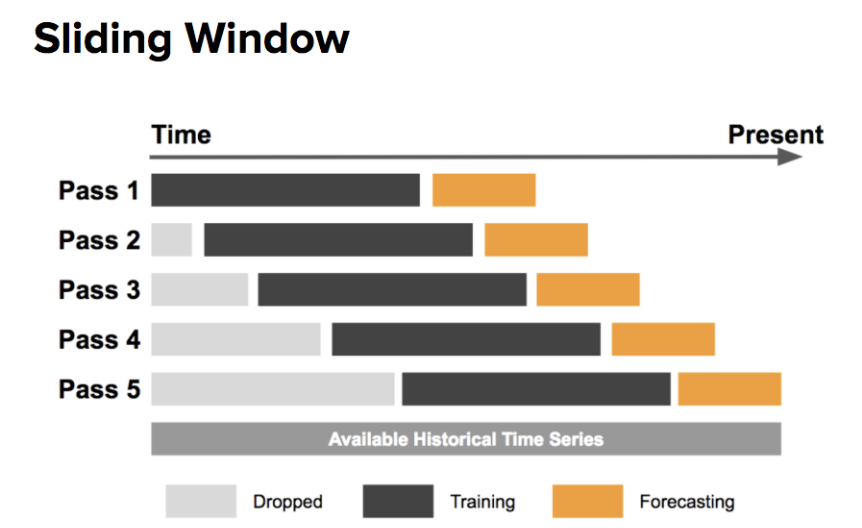
\includegraphics[width=0.6\textwidth]{../figures/uber_backtesting_sliding_window.png}
		\caption{Illustration of rolling (sliding) window CV.}
	\end{figure}
	\medskip

	For each pass, we train on a portion of the data and test on the next time period, then slide forward. For obtain multiple $h$-step forecasts which can be evaluated against actual values.
\end{frame}


\begin{frame}{Example for two test-training splits}
	\begin{figure}
		\centering
		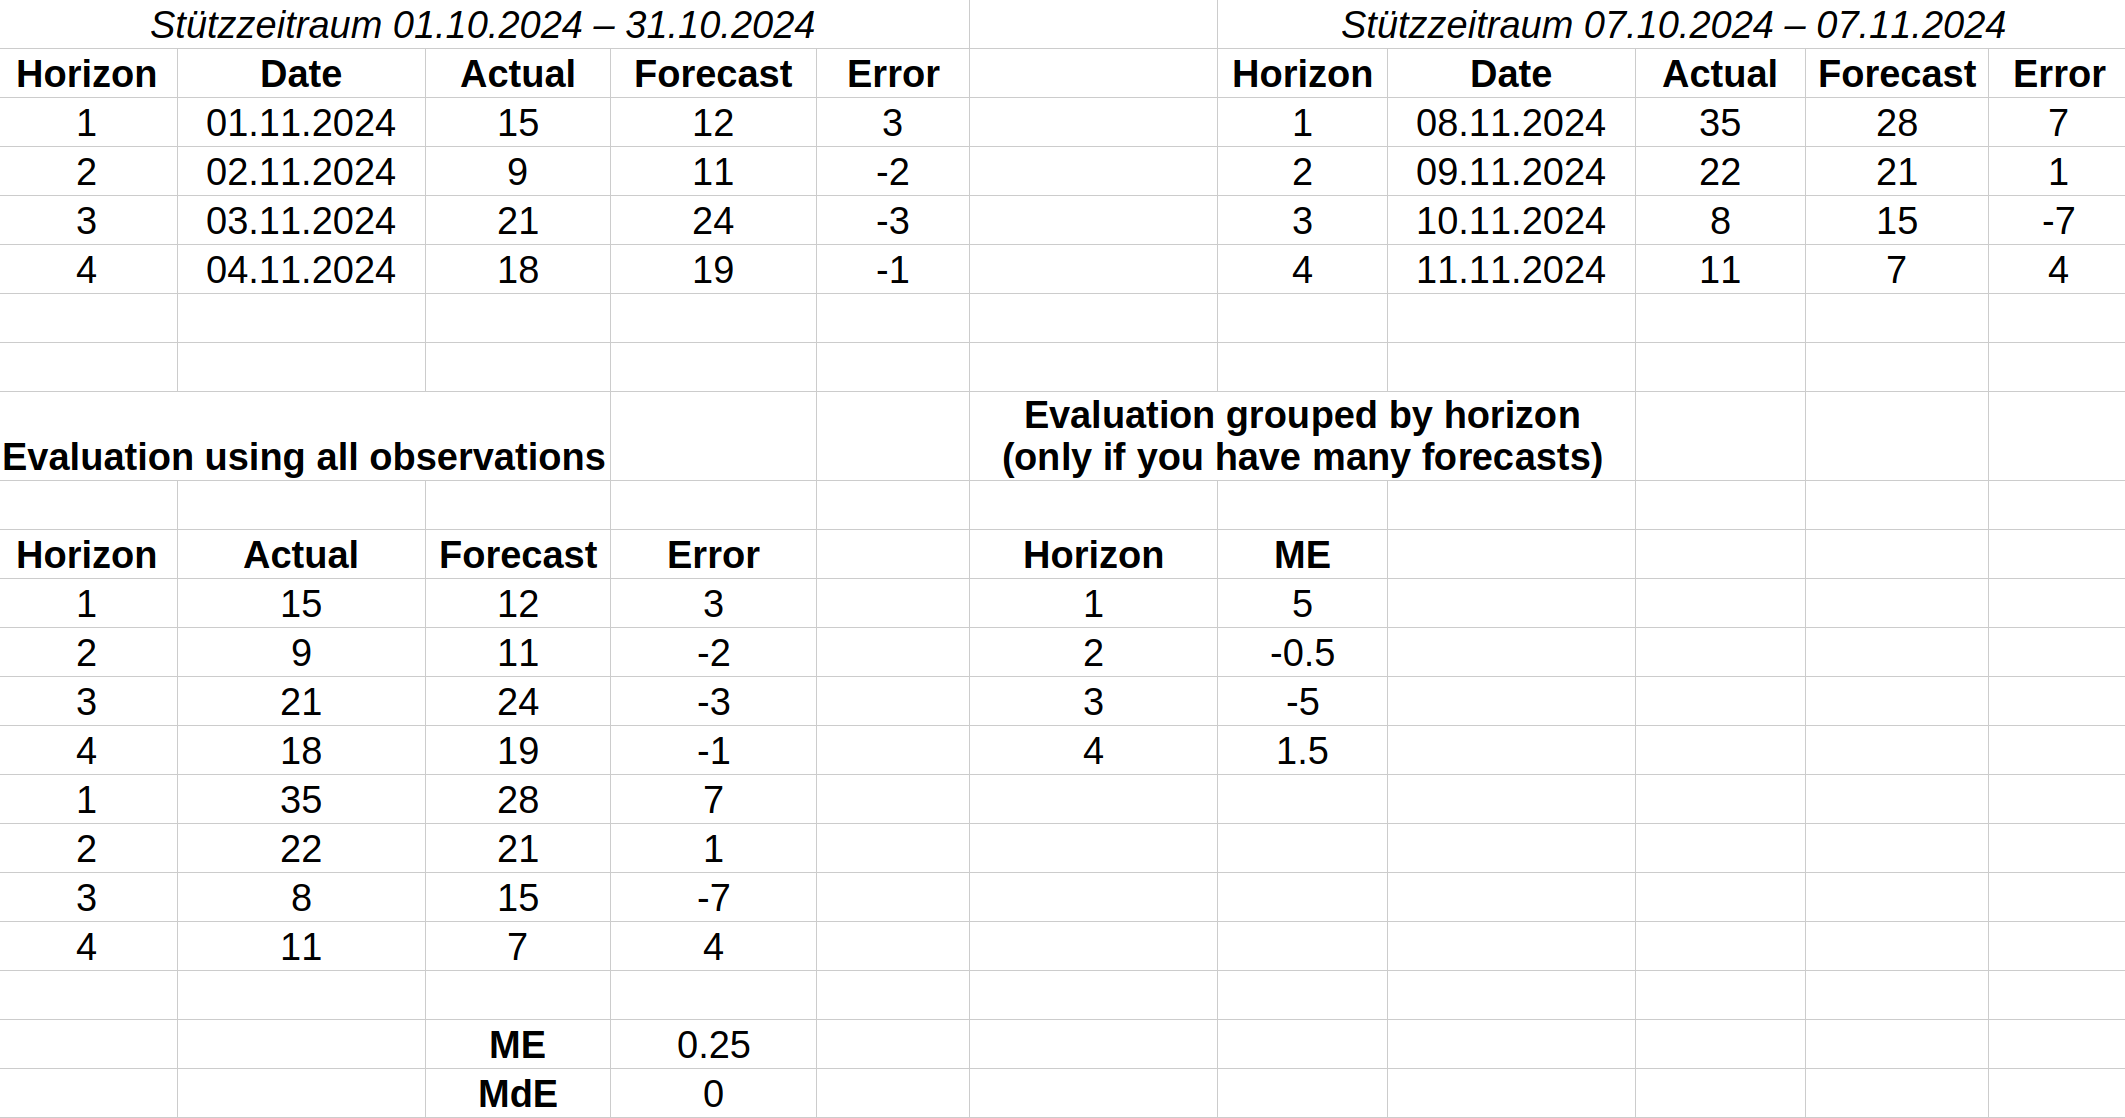
\includegraphics[width=1.0\textwidth]{../figures/beispiel_evaluation_mehrere_stuetzzeitpunkte.png}
		\caption{Evaluation of 4-step forecasts using two different test-training splits.}
	\end{figure}
\end{frame}


\begin{frame}{Cross-validation: Example in Beer Production}
    \begin{columns}[T]
        \column{0.3\textwidth}
        \textbf{Key points}
        \begin{itemize}
            \item Five models
            \item Rolling window CV with window size 50 quarters
            \item $k=24$ test-training splits (each with 8-step forecasts)
            \item In total 164 forecasts per model $\Rightarrow$ 164 forecast errors for evaluation
        \end{itemize}

        \column{0.7\textwidth}
        \begin{table}
            \centering
            \tiny
            \resizebox{\textwidth}{!}{
                \begin{tabular}{lrrrrr}
                    \toprule
                    & \textbf{Seas. model} & \textbf{Seas. mean} & \textbf{RW} & \textbf{RW+drift} & \textbf{AR(1)} \\
                    \midrule
                    \textbf{ME}   & -9.52 & 2.00  & 0.55  & 2.18  & \textbf{1.99}  \\
                    \textbf{RMSE} & \textbf{14.89} & 15.22 & 50.64 & 54.41 & 15.70 \\
                    \textbf{MAE}  & 11.97 & \textbf{11.96} & 39.76 & 43.01 & 12.36 \\
                    \textbf{MPE}  & -2.20 & 0.37  & -0.60 & \textbf{-0.21} & 0.36  \\
                    \textbf{MAPE} & \textbf{2.79}  & 2.80  & 9.26  & 10.02 & 2.89  \\
                    \bottomrule
                \end{tabular}
            }
        \end{table}

        %\vspace{0.2cm}
        \begin{figure}
            \centering
            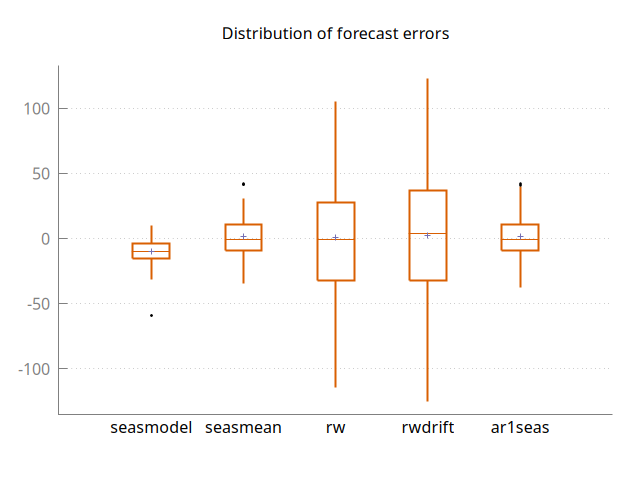
\includegraphics[width=0.7\textwidth]{../figures/boxplot_cross_validated_fcerrors.png}
            \caption{Cross-validation results across rolling windows}
        \end{figure}
    \end{columns}
\end{frame}


% \begin{frame}{Many Forecasting Methods Exist}
% 	\begin{figure}
% 		\centering
% 		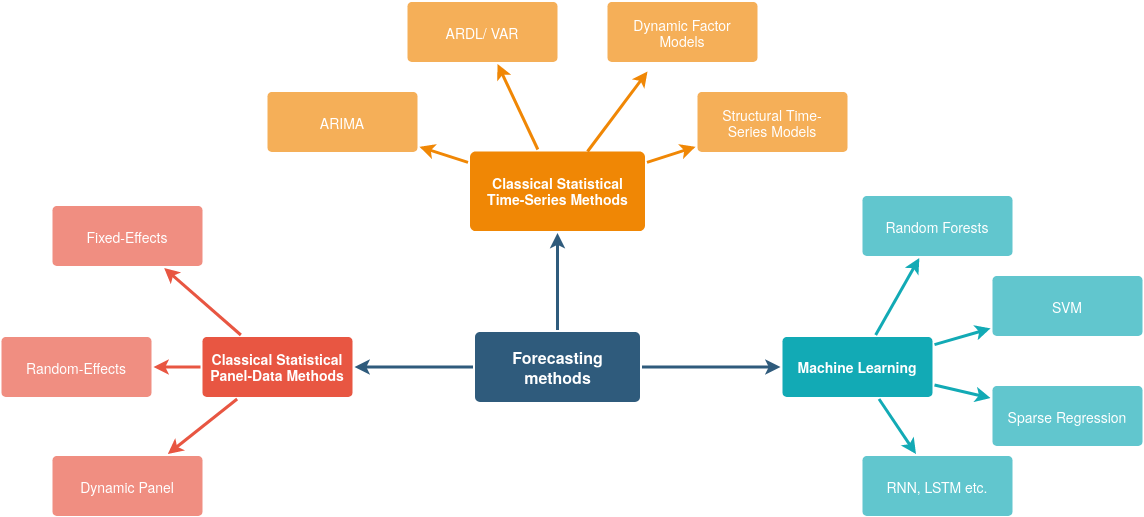
\includegraphics[width=0.9\textwidth]{../figures/Forecasting_methods.png}
% 		\caption{Many forecasting methods exist, from simple benchmarks to complex machine learning models.}
% 		\label{fig:forecasting_methods}
% 	\end{figure}
% \end{frame}



% ==================== SECTION 5: DYNAMIC MODELS ====================

% \section{Dynamic Model Forecasts: ARIMA}

% \begin{frame}
% 	\begin{center}
% 		\Large
% 		Dynamic Model Forecasts: ARIMA
% 	\end{center}
% \end{frame}

% \begin{frame}[fragile]{When Do Naive Methods Fail?}
% 	\begin{itemize}
% 		\item Data with \textbf{autocorrelation}: Past values contain predictive info
% 		\item \textbf{Complex patterns}: Trends, level shifts, cycles
% 		\item \textbf{Structural dependencies}: Future depends systematically on past
% 	\end{itemize}

% 	\vspace{0.5cm}
% 	\textbf{Solution:} Use data patterns to improve forecasts

% 	\vspace{0.5cm}
% 	\textbf{Introducing ARIMA:}
% 	\begin{itemize}
% 		\item \textbf{A}uto\textbf{R}egressive: Uses past values
% 		\item \textbf{I}ntegrated: Handles non-stationarity via differencing
% 		\item \textbf{M}oving \textbf{A}verage: Uses past forecast errors
% 	\end{itemize}
% \end{frame}

% \begin{frame}[fragile]{ARIMA Components I: AutoRegressive (AR)}
% 	\textbf{Idea:} Forecast based on past values of the series
% 	$$y_t = c + \phi_1 y_{t-1} + \phi_2 y_{t-2} + \cdots + \phi_p y_{t-p} + e_t$$

% 	\vspace{0.3cm}
% 	\begin{itemize}
% 		\item Parameter $p$ = number of lags (AR order)
% 		\item $\phi_i$ = coefficients (how much past values matter)
% 		\item Works well when: Past behavior predicts future behavior
% 	\end{itemize}

% 	\vspace{0.5cm}
% 	\textbf{Example AR(1):}
% 	$$y_t = 0.7 y_{t-1} + e_t$$
% 	\begin{itemize}
% 		\item Today's value = 70\% of yesterday's value + random shock
% 		\item Exhibits autocorrelation and mean reversion
% 	\end{itemize}
% \end{frame}

% \begin{frame}[fragile]{ARIMA Components II: Integrated (I)}
% 	\textbf{Problem:} Many economic series are non-stationary (trending)

% 	\vspace{0.5cm}
% 	\textbf{Solution:} Differencing to remove trend
% 	$$\Delta y_t = y_t - y_{t-1}$$

% 	\vspace{0.3cm}
% 	Parameter $d$ = number of differences needed for stationarity
% 	\begin{itemize}
% 		\item $d=0$: Already stationary (use AR/MA directly)
% 		\item $d=1$: First difference needed (most common)
% 		\item $d=2$: Second difference (rare, usually overkill)
% 	\end{itemize}

% 	\vspace{0.5cm}
% 	\textbf{Stationarity check:}
% 	\begin{itemize}
% 		\item ADF test: Does series have unit root?
% 		\item ACF plot: How long does autocorrelation persist?
% 	\end{itemize}
% \end{frame}

% \begin{frame}[fragile]{ARIMA Components III: Moving Average (MA)}
% 	\textbf{Idea:} Forecast based on past forecast \remph{errors}
% 	$$y_t = \mu + e_t + \theta_1 e_{t-1} + \theta_2 e_{t-2} + \cdots + \theta_q e_{t-q}$$

% 	\vspace{0.3cm}
% 	\begin{itemize}
% 		\item Parameter $q$ = number of error lags (MA order)
% 		\item $\theta_i$ = error coefficients
% 		\item Helps smooth out ``shocks''
% 	\end{itemize}

% 	\vspace{0.5cm}
% 	\textbf{Key insight:} MA captures short-term deviations, AR captures persistence
% \end{frame}

% \begin{frame}[fragile]{ARIMA Notation and Identification}
% 	\textbf{ARIMA(p, d, q):}
% 	\begin{itemize}
% 		\item $p$ = AR order (lags of dependent variable)
% 		\item $d$ = Differencing (for stationarity)
% 		\item $q$ = MA order (lags of errors)
% 	\end{itemize}

% 	\vspace{0.5cm}
% 	\textbf{Examples:}
% 	\begin{itemize}
% 		\item ARIMA(1,0,0) = AR(1): Autoregressive, no differencing
% 		\item ARIMA(0,1,0) = Random walk: First difference only
% 		\item ARIMA(0,1,1) = Simple exponential smoothing
% 		\item ARIMA(1,1,1) = Combination of all three
% 	\end{itemize}

% 	\vspace{0.5cm}
% 	\textbf{Seasonal extension:} ARIMA(p,d,q)(P,D,Q)$_s$ for seasonal patterns
% \end{frame}

% \begin{frame}[fragile]{Identifying ARIMA Orders}
% 	\textbf{Step 1: Check stationarity}
% 	\begin{itemize}
% 		\item ADF test: Null = unit root (non-stationary)
% 		\item If not stationary, set $d=1$ and retest
% 	\end{itemize}

% 	\vspace{0.3cm}
% 	\textbf{Step 2: Determine $p$ from PACF (Partial Autocorrelation)}
% 	\begin{itemize}
% 		\item Count significant spikes in PACF $\Rightarrow$ suggests $p$
% 	\end{itemize}

% 	\vspace{0.3cm}
% 	\textbf{Step 3: Determine $q$ from ACF (Autocorrelation)}
% 	\begin{itemize}
% 		\item Count significant spikes in ACF $\Rightarrow$ suggests $q$
% 	\end{itemize}

% 	\vspace{0.5cm}
% 	\textbf{Alternative:} Use automatic model selection (AIC/BIC)
% \end{frame}

% \begin{frame}[fragile]{Direct vs. Recursive Forecasting}
% 	\textbf{Recursive (Dynamic) Method:}
% 	\begin{itemize}
% 		\item Generate $h$-step forecast using model dynamics
% 		\item Each forecast step uses previously forecasted value
% 		\item Captures autoregressive structure
% 		\item Better for medium/long horizons
% 	\end{itemize}

% 	\vspace{0.5cm}
% 	\textbf{Direct Method:}
% 	\begin{itemize}
% 		\item Fit separate model for each horizon $h$
% 		\item More computationally intensive
% 		\item Can lack continuity between horizons
% 	\end{itemize}

% 	\vspace{0.5cm}
% 	\textbf{Recommendation:} Use recursive forecasting for ARIMA (default in most software)
% \end{frame}

% \begin{frame}[fragile]{ARIMA in Gretl: Estimation}
% 	\textbf{Step 1: Test for stationarity}
% 	\begin{verbatim}
% adf y  # Augmented Dickey-Fuller test
% 	\end{verbatim}

% 	\vspace{0.3cm}
% 	\textbf{Step 2: Examine ACF/PACF}
% 	\begin{verbatim}
% corrgm y 24 --plot  # Correlogram for 24 lags
% 	\end{verbatim}

% 	\vspace{0.3cm}
% 	\textbf{Step 3: Fit ARIMA model}
% 	\begin{verbatim}
% arima 1 1 1; y  # ARIMA(1,1,1)
% 	\end{verbatim}

% 	\vspace{0.3cm}
% 	\textbf{Step 4: Check residuals}
% 	\begin{verbatim}
% corrgm $uhat 24  # Should be white noise
% 	\end{verbatim}
% \end{frame}

% \begin{frame}[fragile]{ARIMA in Gretl: Forecasting}
% 	\textbf{Generate forecasts with confidence intervals:}
% 	\begin{verbatim}
% arima 1 1 1; y
% fcast 2018:1 2018:4  # Forecast 4 quarters ahead
% 	\end{verbatim}

% 	\vspace{0.5cm}
% 	\textbf{Output:} Point forecast + standard error (for intervals)

% 	\vspace{0.5cm}
% 	\textbf{Recursive forecasting:} Automatic in Gretl's ARIMA
% 	\begin{itemize}
% 		\item Each step uses previous forecast when needed
% 	\end{itemize}
% \end{frame}

% \begin{frame}[fragile]{Comparing Forecasting Methods}
% 	\begin{figure}
% 		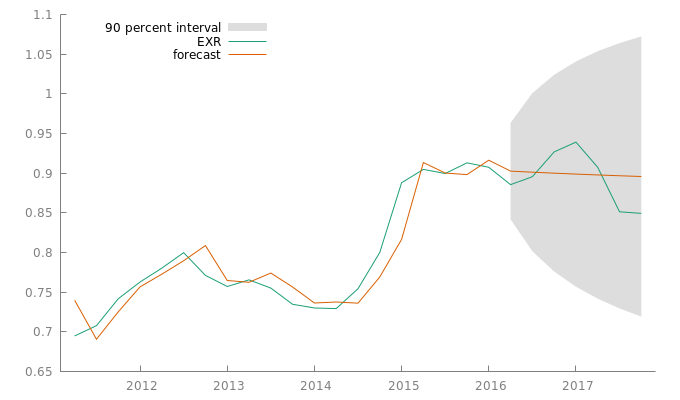
\includegraphics[width=0.7\textwidth]{../figures/arma_11_prognose_exr.png}
% 		\caption{ARIMA vs. simple methods: When does sophistication pay off?}
% 	\end{figure}

% 	\textbf{Key insight:} ARIMA better when autocorrelation is strong; naive otherwise
% \end{frame}

% % ==================== SECTION 6: SUMMARY ====================

% \section{Summary and Key Takeaways}

% \begin{frame}
% 	\begin{center}
% 		\Large
% 		Summary and Key Takeaways
% 	\end{center}
% \end{frame}

% \begin{frame}[fragile]{Forecasting Best Practices}
% 	\begin{enumerate}
% 		\item \textbf{Start simple}: Begin with naive methods as benchmark
% 		      \begin{itemize}
% 			      \item If complex methods don't beat naive, use naive!
% 		      \end{itemize}

% 		\item \textbf{Always evaluate on test set}: Never use training metrics
% 		      \begin{itemize}
% 			      \item Separate data before any modeling
% 		      \end{itemize}

% 		\item \textbf{Use appropriate metrics}: MASE for comparing methods
% 		      \begin{itemize}
% 			      \item MASE < 1 means better than naive forecast
% 		      \end{itemize}

% 		\item \textbf{Include uncertainty}: Report prediction intervals, not just point forecasts

% 		\item \textbf{Validate with cross-validation}: Use expanding/sliding windows for time series

% 		\item \textbf{Keep it interpretable}: Simpler models usually beat complex ones
% 	\end{enumerate}
% \end{frame}

% \begin{frame}[fragile]{When to Use Each Method}
% 	\begin{itemize}
% 		\item \textbf{Mean}: Stationary, no trend or seasonality

% 		\item \textbf{Naïve}: Random walk (most financial/macro data)

% 		\item \textbf{Seasonal Naïve}: Strong seasonal patterns (retail, energy)

% 		\item \textbf{Drift}: Steady trend (GDP, population)

% 		\item \textbf{ARIMA}: Strong autocorrelation, need to capture dynamics
% 		      \begin{itemize}
% 			      \item Check ADF test and ACF/PACF first
% 		      \end{itemize}
% 	\end{itemize}

% 	\vspace{0.5cm}
% 	\textbf{Rule of thumb:} Seasonal Naïve beats ARIMA more often than you'd expect!
% \end{frame}

% \begin{frame}[fragile]{Key Insights}
% 	\begin{itemize}
% 		\item \textbf{Naive methods are hard to beat}
% 		      \begin{itemize}
% 			      \item Many "sophisticated" methods fail this basic test
% 		      \end{itemize}

% 		\item \textbf{Forecast intervals matter as much as point forecasts}
% 		      \begin{itemize}
% 			      \item Decision-makers need uncertainty estimates
% 		      \end{itemize}

% 		\item \textbf{Simple $\neq$ Bad}
% 		      \begin{itemize}
% 			      \item Parsimony principle: choose simplest model that explains data
% 		      \end{itemize}

% 		\item \textbf{Evaluation is crucial}
% 		      \begin{itemize}
% 			      \item Out-of-sample performance is what matters
% 		      \end{itemize}

% 		\item \textbf{Context matters}
% 		      \begin{itemize}
% 			      \item Economic knowledge helps identify right patterns
% 		      \end{itemize}
% 	\end{itemize}
% \end{frame}

% Load bibliography
\setcounter{secnumdepth}{0}


%% IF YOU USE BIBER
%\begin{frame}[allowframebreaks]{References}
\begin{frame}{References}
\printbibliography
\end{frame}

%% IF YOU USE NATBIB
%\addcontentsline{toc}{section}{REFERENCES}

% \begin{frame}[allowframebreaks]
% 	\frametitle{References}
% 	\small
% 	%\bibliographystyle{quarterly}
% 	%\bibliographystyle{dinat}
% 	\bibliographystyle{cje}
% 	\bibliography{/home/admin-tarassow/Nextcloud/thb_bwsyncandshare/LiteraturVerwaltung/library}
% \end{frame}


\appendix
\setcounter{framenumber}{0}

\section{Appendix}

\begin{frame}{}
	\begin{center}
		\Large
		Appendix

		---

		Additional Material and Examples
	\end{center}
\end{frame}


\begin{frame}{Forecasting, Goals, and Planning}
	\begin{columns}[T]
		\column{0.5\textwidth}
		\textbf{Forecasts}
		\begin{itemize}
			\item Are frequent statistical tasks in business
			\item Help inform decisions about planning production, transport, and staffing
			\item Provide guidance for long-term strategic planning
			\item Business forecasting is often done poorly % and frequently confused with planning and goals
		\end{itemize}

		\column{0.5\textwidth}
		\textbf{What's forecasted?}
		\begin{itemize}
			\item \textbf{Economics}: GDP growth, inflation, unemployment
			\item \textbf{Finance}: Stock prices, exchange rates, asset returns
			\item \textbf{Operations}: Demand forecasting, inventory management, staffing
			\item \textbf{Planning}: Budget allocation, resource allocation, risk management
		\end{itemize}
	\end{columns}
\end{frame}

\begin{frame}{Forecasting, Goals, and Planning}
	\begin{block}{Forecast}
		Seeks to predict the future as accurately as possible, taking into account all available information, including historical data and knowledge of future events that may influence forecasts.
	\end{block}

	\begin{block}{Goals}
		Goals are what you would like to achieve. Goals should be linked to forecasts and plans, but often are not.

		Too often, goals are set without a plan for how to achieve them, and without forecasts of whether they are realistic.
	\end{block}

	\begin{block}{Planning}
		Is a response to forecasts and goals. Planning involves determining the appropriate actions required to align your forecasts with your goals.
	\end{block}
\end{frame}

\begin{frame}{Naive/simple methods as special cases of ARIMA}
	\textbf{ARIMA(p, d, q):}
	\begin{itemize}
		\item $p$ = AR order (lags of dependent variable)
		\item $d$ = Differencing (for stationarity)
		\item $q$ = MA order (lags of errors)
	\end{itemize}

	\vspace{0.15cm}
	\textbf{Examples:}\footnote{See, e.g., \url{https://otexts.com/fpp3/non-seasonal-arima.html}}
	\begin{itemize}
		\item ARIMA(0,0,0) = White noise with no constant
		\item ARIMA(p,0,0) = AR(p): Autoregressive, no differencing
		\item ARIMA(0,1,0) = Random walk without drift (no constant)
		\item ARIMA(0,1,0) = Random walk with drift (with constant)
		\item ARIMA(0,1,1) = Simple exponential smoothing
		%\item ARIMA(1,1,1) = Combination of all three
	\end{itemize}

	\vspace{0.1cm}
	\textbf{Seasonal extension:} ARIMA(p,d,q)(P,D,Q)$_s$ for seasonal patterns.
\end{frame}

\begin{frame}[fragile]{Cross-Validation Approaches}
	\textbf{Expanding Window (preferred):}
	\begin{itemize}
		\item Training set grows, test set fixed
		\item Mimics real-world forecasting: more data accumulates over time
		\item Better for stable models
	\end{itemize}

	\vspace{0.5cm}
	\textbf{Sliding Window:}
	\begin{itemize}
		\item Fixed training size slides forward
		\item Test set moves with training set
		\item Better if model performance changes over time
	\end{itemize}

	\vspace{0.5cm}
	\textbf{Gretl implementation:} Manual backtesting loop with forecast generation
\end{frame}

\end{document}
